\chapter{Voice Onset Time}\label{sec:VOT}

The following figures show the voice onset times of several consonants in initial and intervocalic positions. The pitch contour can be used as an indicator of voicing: without voice, there is no pitch. The formants indicate the vocalic phases. The offset between  the beginning of the pitch contour and the beginning of the vocalic phase is taken here as the determinant of voice onset time.

Generally speaking, SLM voiceless stops have a voice onset time of close to 0ms. Voiced stops have a negative VOT, and tend to be fully voiced, i.e. the voicing does not cease between vowels preceding and following the voiced stop.

An interesting fact is that voiced stops tend to have a negative VOT even if they follow the voiceless fricative /s-/.

The figures were selected to cover a maximum of the parametric variation possible for [$\pm$voicing], [$\pm$geminate], [$\pm$initial], [$\pm$ intervocalic], and [$\pm$following s].

% \paragraph{VOT in the onset}
\begin{figure*}
 \centering
 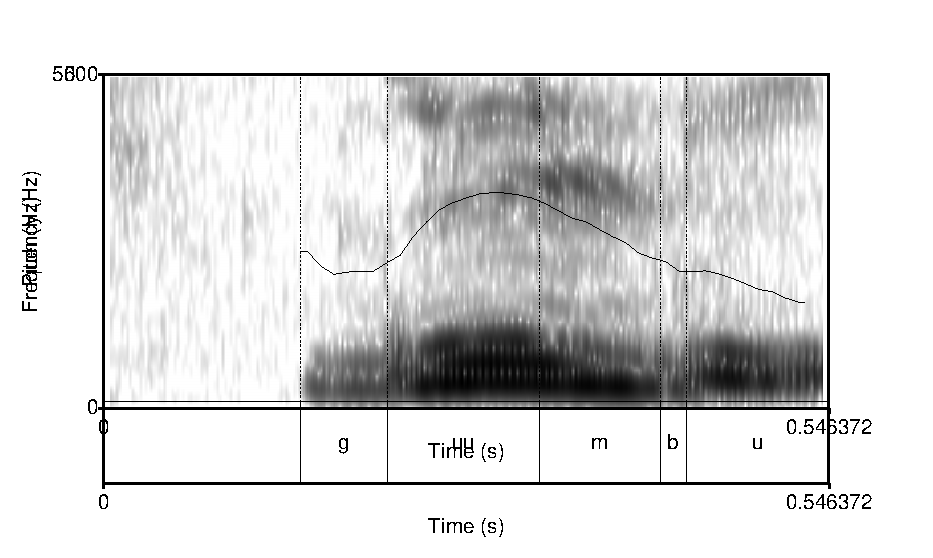
\includegraphics[height=0.3\textheight]{./pics/guumbu-a.eps}

 \includegraphics[height=0.3\textheight]{./pics/inithumpathpadayam.eps}

 \caption[VOT of /g,\dentt, p/ in onsets]{[g] in the absolute onset of \phontrs{gu:\umb u}{Negombo (town)} is fully voiced and has a negative VOT of about 0.068s (above). This can be seen from the pitch contour, which is present during the whole articulation of g. Since pitch can only be measured on voiced parts, the pitch contour can be used to identify voicing. The image below shows that the pitch contour is absent for  [\dentt] and [p], but voicing sets in as soon as closure of the mouth is released and the vocalic part begins, i.e. we  have a voice onset time of close to zero in the onsets [\dentt u-, pa-, pa-].}
 \label{fig:phon:vot:inithumpathpadayam}
\end{figure*}

\begin{figure*}
 \centering
 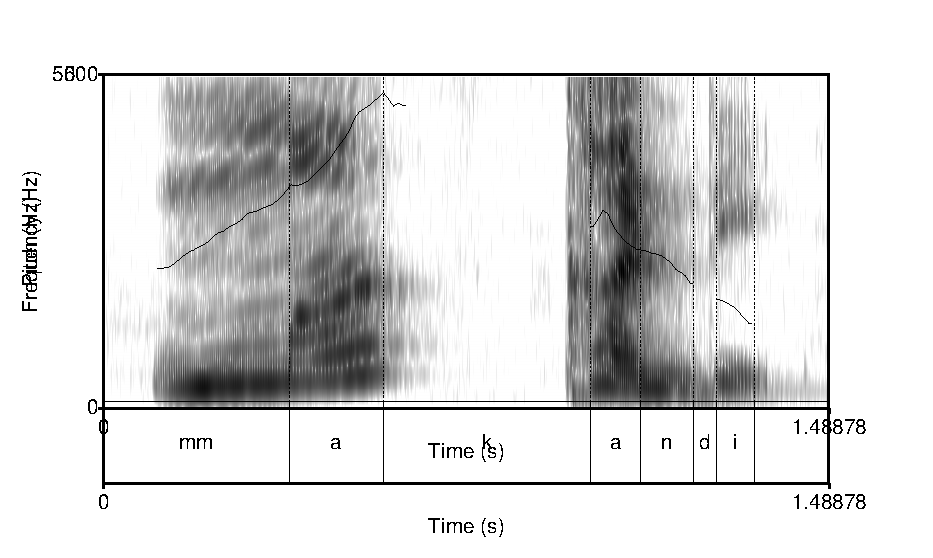
\includegraphics[height=0.3\textheight]{./pics/mmakandi-asp.eps}
 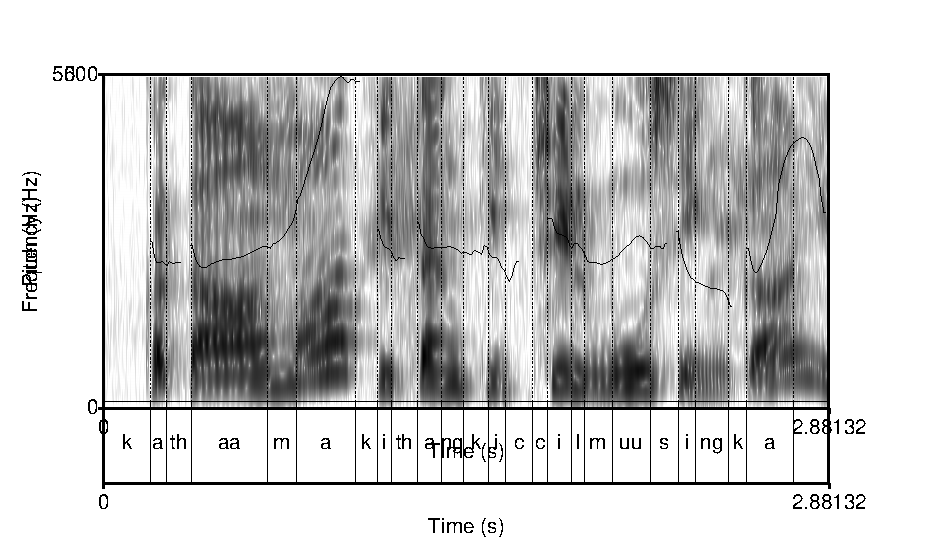
\includegraphics[height=0.3\textheight]{./pics/kathaamakiccilmuusingka.eps}

 \caption[VOT of rare aspirated /k/ and comparison with the normal, non-aspirated case.]{It is rare to find aspirated consonants in SLM, identified by long VOTs, like the [k] in \phontrs{ka\postalvn\postalvd i}{Kandy (town)} the example above, which has a VOT of 0.049s. One can see from the black shading that the closure is already released, but the voicing has not started yet (indicated by the pitch line).
It is much more common to have VOTs under 0.020s, as is the case with all the stops in the example below.}
 \label{fig:phon:vot:mmakang-asp}
\end{figure*}

% \paragraph{VOT in intervocalic position}
\begin{figure*}
 \centering
 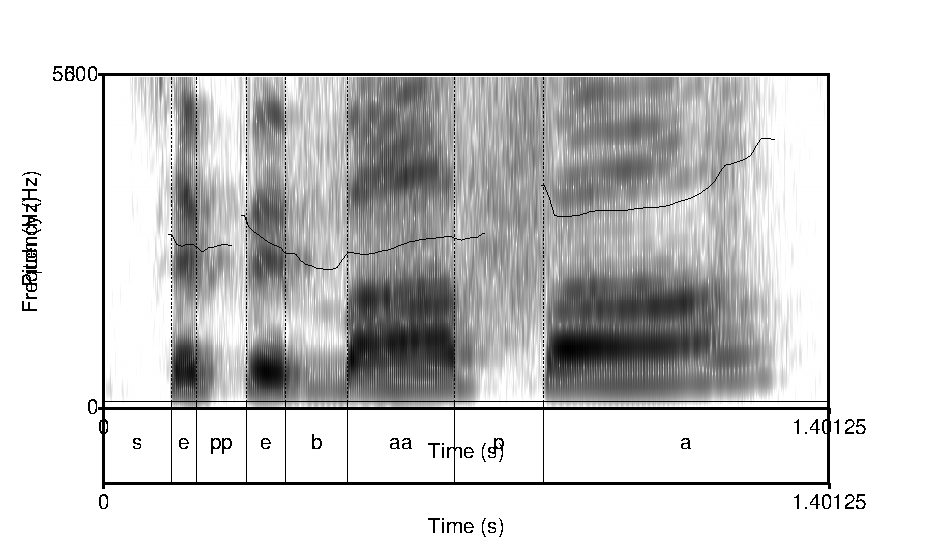
\includegraphics[height=0.3\textheight]{./pics/seppebaapa.eps}
 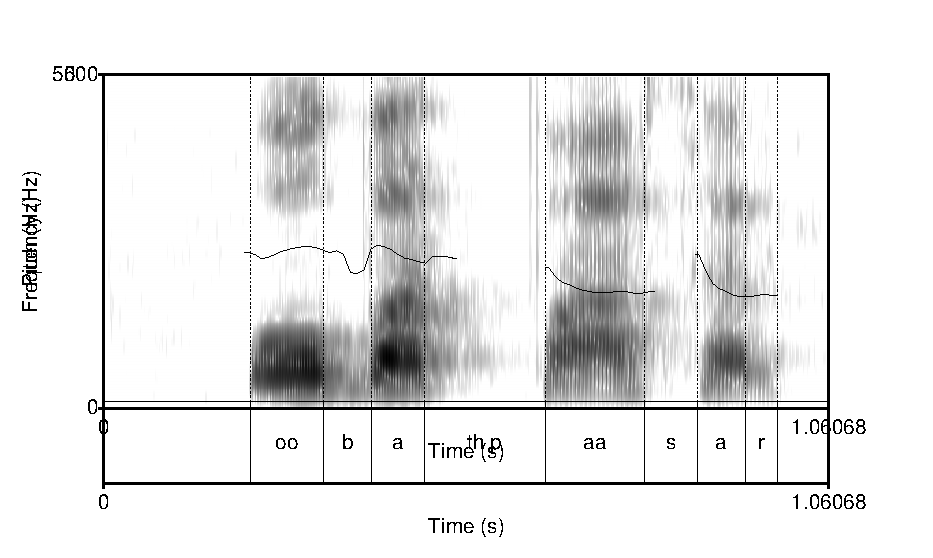
\includegraphics[height=0.3\textheight]{./pics/oobathpaasar.eps}
 \caption[VOT of intervocalic /p/ and /b/]{[p] in intervocalic position [a:pa] has a VOT close to zero. [b] in intervocalic position between two morphemes is fully voiced. (above). [b] in morpheme-internal intervocalic position is fully voiced, /p/ in the onset of [pa:sar] has a VOT close to zero (below).}
 \label{fig:phon:vot:oobathpaasar}
\end{figure*}

% \paragraph{VOT in intervocalic position, geminated}


\begin{figure*}
 \centering
 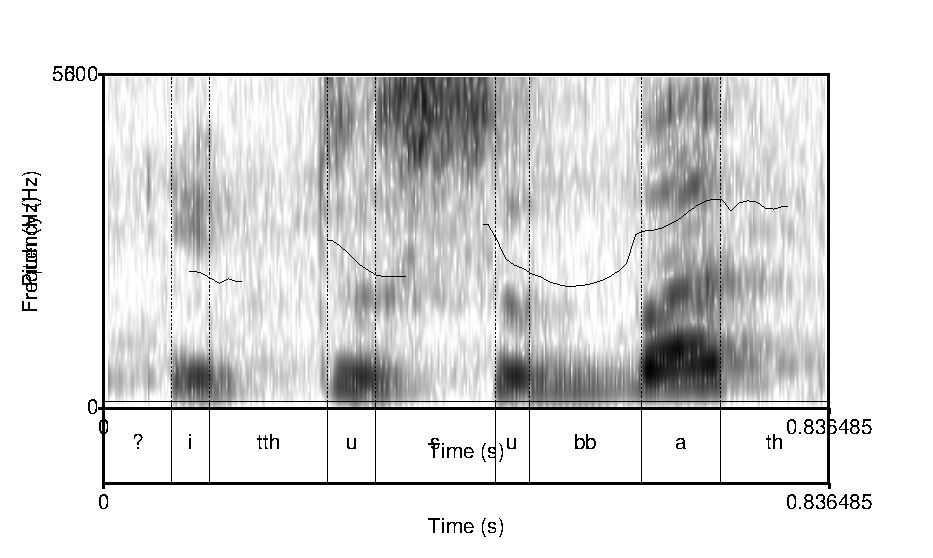
\includegraphics[height=0.3\textheight]{./pics/itthusubbath.eps}
%
 \caption[VOT of geminate /\dentt:/ and /b:/]{The  long dental stop in [i\dentt:u] has a VOT close to zero, the  long labial stop in [sub:a\dentt] is fully voiced.}
 \label{fig:phon:vot:itthusubbath}
\end{figure*}



% \paragraph{VOT after /s-/}

\begin{figure*}
 \centering
 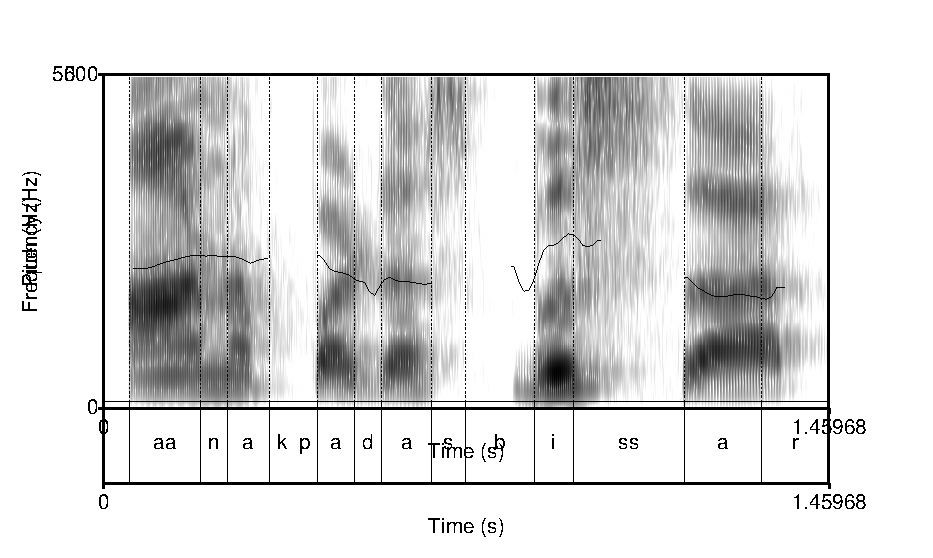
\includegraphics[height=0.3\textheight]{./pics/sbissar.eps}

 \caption[VOT of /b/ after /s/]{Even after the voiceless fricative [s-], /b/  has a negative VOT of -0.045s. [p] in [pada] has a VOT close to zero.}
 \label{fig:phon:vot:bissar}
\end{figure*}


\begin{figure*}
 \centering
 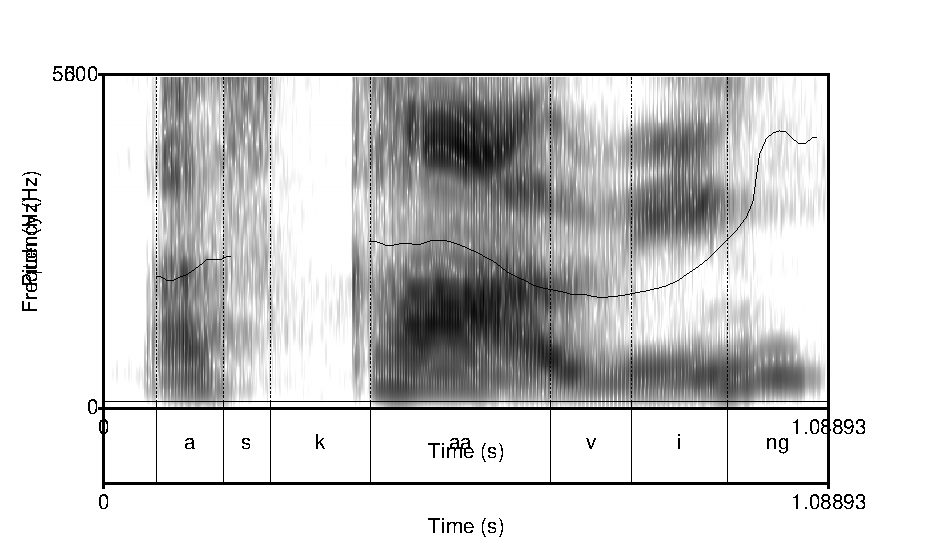
\includegraphics[height=0.3\textheight]{./pics/askaaving.eps}

 \caption[VOT of /k/ after /s/]{After the voiceless fricative /s/, [k] has a VOT of 0.027s.}
 \label{fig:phon:vot:askaaving}
\end{figure*}

% 
% \begin{table}
% \begin{center}
% % use packages: array
% \begin{tabular}{lllll}
%  & initial & intervocalic & geminated & following s- \\
% voiced &  &  &  &  \\ 
% voiceless &  &  &  & 
% \end{tabular}
% \end{center}
% \caption{Voice onset times for different environments}
% \label{tab:phon:VOT}
% \end{table}
